% 3.1: definition of online perception; limitation of Rec and SV; our idea: extend SV to Online, take advantages of both: 1) online ability; 2) high performance on whole scene
% 3.2: Memory construction
% 3.3: Memory-based adapter
% 3D memory can be long due to space is limited. While 2D memory is short.

In this section, we first introduce the definition of online 3D scene perception and explain our motivation of memory-based adapter. Then we describe how to construct memory and refine the backbone features by adapter for point cloud and image respectively.

\subsection{Online 3D Scene Perception}\label{def}
Let $\mathcal{X}_t=\{x_1,x_2,...,x_t\}$ be a posed RGB-D streaming video, which means the video is collected with the moving of sensor rather than a pre-collected video. We have:
\begin{equation}
    x_t=(I_t,P_t,M_t),\ I_t\in \mathbb{R}^{H\times W\times 3},\ P_t\in \mathbb{R}^{N\times 3},\ M_t\in \mathbb{R}^{3\times 4}
\end{equation}
where $I_t$ and $P_t$ refer to the image and point clouds for one RGB-D frame. $P_t$ is acquired by lifting the depth image to world coordinate system with pose parameters $M_t$, where $M_t$ can be estimated by visual odometry~\cite{park2017colored,zhao2021surprising}.
At time $t$, the input to online perception model is $\mathcal{X}_t$ and the output is predictions for the observed 3D scene $S_t=\bigcup_{i=1}^t{P_i}$, which can be bounding boxes and semantic/instance masks. Some works also perform 3D reconstruction along with online perception~\cite{liu2022ins} to acquire high-quality point clouds or meshes, but this is not required~\cite{chaplot2020object,ramakrishnan2022poni,zhang20233d}. In this work we do not rely on 3D reconstruction and directly take RGB-D streaming video as input, which is a more general setting.

% better explain the second paragraph
% figures, insseg is good
% training scene / 10 / ALL
% M_rec: training scene / x / x
% M_SV: training scene / x / x
Although great improvement has been achieved in the design of 3D perception models, most of them only focus on two scenarios: (1) Reconstructed scenes~\cite{armeni20163d,dai2017scannet}. The model $\mathcal{M}_{Rec}$ is trained on point clouds of complete scenes reconstructed from RGB-D videos. (2) Single-view scenes~\cite{Silberman2012nyu,song2015sun}. The model $\mathcal{M}_{SV}$ is trained on single-view point clouds back-projected from RGB-D image. However, $\mathcal{M}_{Rec}$ requires the input to be a complete scene, which is not accessible in real-time tasks. $\mathcal{M}_{SV}$ is able to process RGB-D videos frame-by-frame, but fails to exploit temporal information. 
Therefore, previous 3D models are not ready for the more practical online scene perception.

To this end, we aim to devise a plug-and-play temporal learning module, which can be inserted into any single-view perception model $\mathcal{M}_{SV}$ and empowers it with temporal modeling ability. 
Note that $\mathcal{M}_{SV}$ is originally a 3D perception model. We can extend it to a RGB-D perception model by early fusing the image features to point clouds~\cite{rukhovich2023tr3d}:
\begin{gather}
    p_t=\mathcal{M}_{SV}(P'_t), \nonumber \\
    P'_t=P_t\oplus \mathcal{S}(\mathcal{M}_I(I_t),P_t,M_t),\ \mathcal{S}(\cdot)\in \mathbb{R}^{N\times C}
\end{gather}
where $p_t$ is the prediction for input frame at time $t$. $\mathcal{M}_I$ is a image backbone pretrained on the same perception task as $\mathcal{M}_{SV}$. $\mathcal{S}$ projects $P_t$ to image coordinate system by $M_t$ and samples the corresponding 2D features to enrich the features of $P_t$.
We divide $\mathcal{M}_{SV}$ into a backbone $\mathcal{M}_{P}$ for extracting features of point clouds and a task-specific head $\mathcal{M}_{H}$. The goal of this work is to construct an image memory-based adapter for $\mathcal{M}_I(I_t)$ and a point cloud memory-based adapter for $\mathcal{M}_{P}(P'_t)$ to store and reuse the extracted backbone features for temporal modeling:
\begin{gather}
    \mathcal{M}_{I}(I_t),m^I_t=\mathcal{A}_I(\mathcal{M}_{I}(I_t),m^I_{t-1},m^P_{t-1}), \nonumber \\
    \mathcal{M}_{P}(P'_t),m^P_t=\mathcal{A}_P(\mathcal{M}_{P}(P'_t),m^P_{t-1})
\end{gather}
where the memory-based adapter $\mathcal{A}$ updates the memory $m_t$ with current features and refines current features by reusing the memory. 
We fully exploit inter-modal and intra-modal relationships: $\mathcal{M}_{SV}$ fuses image features to point clouds, $\mathcal{A}_P$ reuses previous point cloud features to refine current point cloud features, and $\mathcal{A}_I$ reuses previous features from both modal to refine the current image features.
As shown in Figure \ref{over-arch}, we follow the same paradigm to design both modules, which can be easily embedded into image and point cloud backbones to achieve temporal modeling.

\subsection{Temporal Modeling for Point Clouds}
% voxel representation
% VMP
% if constrained, time-sequence queue
% 3D ASPP
Given $\{\mathcal{M}_{P}(P'_{1}),\mathcal{M}_{P}(P'_{2}),...,\mathcal{M}_{P}(P'_{t})\}$ at time $t$, i.e., the sequence of point cloud features extracted from the backbone, we aim to enhance the current features $\mathcal{M}_{P}(P'_{t})$ by exploiting the temporal relations within this sequence. Here we first construct a memory to efficiently cache the point cloud features from different timestamp. Then we aggregate the temporal information from the memory to features at current time $t$ with a plug-and-play adapter.

\begin{figure}[t]
    \centering
    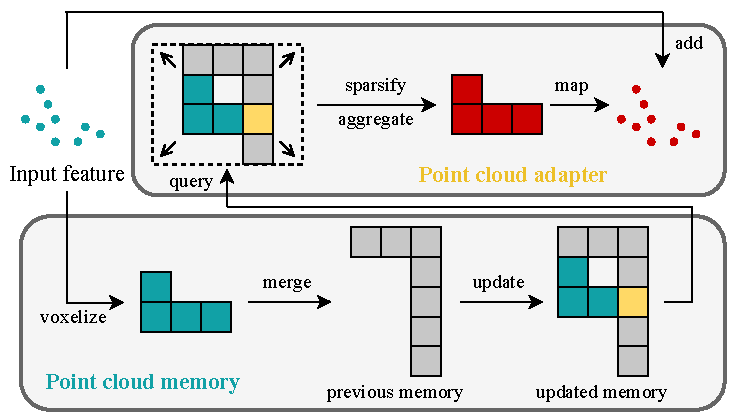
\includegraphics[width=1.0\linewidth]{figures/pc-module-single.pdf}
    \caption{The architecture of the memory-based adapter for point cloud features. We cache and aggregate the features in a queue of 3D voxel grids. Gray, green, yellow and red block refer to previous, current, updated and aggregated voxel features.}
    \label{point-module}
\end{figure}

\textbf{Memory construction:}
The temporal information for 3D scenes is reflected in a more complete geometry. As a single RGB-D frame may not contain a complete large objects or high-level scene context, the geometric information from previous frames are important for accurate perception of current frame. Therefore, we can cache the sequence of extracted point cloud features in a shared 3D space. A simple way is to directly store the features in terms of point clouds in the world coordinate system. However, this is inefficient in both storage and computation: (1) as the coordinates of the point cloud are real values, the storage overhead will keep growing even if the RGB-D camera is not moving; (2) the number of points will be very large over time, so point-based sampling and feature aggregate take up high computation overhead.
To this end, we propose to store the features in a quantitized coordinate system, where point clouds are voxelized and stored in 3D grids. We also maintain the voxels in a queue to reduce the memory footprint when the scene is too large.
Specifically, $\mathcal{M}_{P}(P'_t)$ is first voxelized into the voxel grids $V_t$ by averaging all features whose coordinates falls into the same grid. These voxels are tagged with timestamp $t$. Then we merge $V_t$ to the memory $m^P_{t-1}$ by maxpooling:
\begin{gather}
    m^P_{t}={\rm maxpooling}(V_t,m^P_{t-1}), \nonumber \\
    m^P_{t}={\rm deq}(m^P_{t}, l)\ \ if\ \ N(m^P_{t})>N_{max}
\end{gather}
where ${\rm maxpooling}$ refers to channel-wise maxpooling conducted on each voxel grid, which will update both features and timestamps. ${\rm deq}(\cdot,l)$ means removing voxels with timestamp earlier than $t-l+1$ from the memory. $N(m^P_{t})$ is the number of voxels in the memory.
We utilize maxpooling as it preserves the most discriminative features over time, which is also efficient to compute as only features at time $t-1$ and $t$ are required.


\textbf{Memory-based adapter:}
After caching and updating the point cloud features in voxels, we need to make use of $m^P_{t}$ to enhance $\mathcal{M}_{P}(P'_t)$ with temporal information.
To exploit rich scene context from the memory $m^P_t$ while reduce redundant computation, we first use the coordinates of $V_t$ to query a neighbor voxel set:
\begin{equation}
    \mathcal{N}(V_t)=\{m^P_t[x][y][z]|(x,y,z)\in s*\mathcal{B}(V_t)\}
\end{equation}
where $\mathcal{N}(V_t)$ is the queired neighborhood of $V_t$. $m^P_t[x][y][z]$ refers to the voxel in $m^P_t$ at coordinate $(x,y,z)$. $\mathcal{B}$ is the minimum enclosing axis-aligned bounding box of $V_t$ and $s$ is a scaling factor to enlarge the size of box. In this way, the temporal information which provides supporting geometric information for current frame is collected into this voxel set. 

We then convert $\mathcal{N}(V_t)$ to a sparse tensor~\cite{graham20183d,choy20194d}, which is followed by a 3D sparse convolutional module $\mathcal{A}_P$ to aggregate the context information within $\mathcal{N}(V_t)$ to locations of $V_t$.
Finally we update $\mathcal{M}_{P}(P'_t)$ in an adapter-manner: (1) We map the aggregated features back to the coordinates of $\mathcal{M}_{P}(P'_t)$ and then add it to the original features with residual connection; (2) The adapter module $\mathcal{A}_P$ is zero-initialized. Therefore after inserting the adapter, finetuning will smoothly start from the original point.


\subsection{Temporal Modeling for Images}
% follow the same paradigm as 3D
% cannot store in a shared space like 3D
% video analysis
% memory: normal queue-->length to be 1, reorg, shift channels
% adapter: concat with previous memory, 2d conv
For the sequence of image features $\{\mathcal{M}_{I}(I_1),...,\mathcal{M}_{I}(I_t)\}$ at time $t$, we follow the same paradigm as the point cloud counterpart to store it with a memory and aggregate temporal information to current frame $\mathcal{M}_{I}(I_t)$ with an adapter.

\begin{figure}[t]
    \centering
    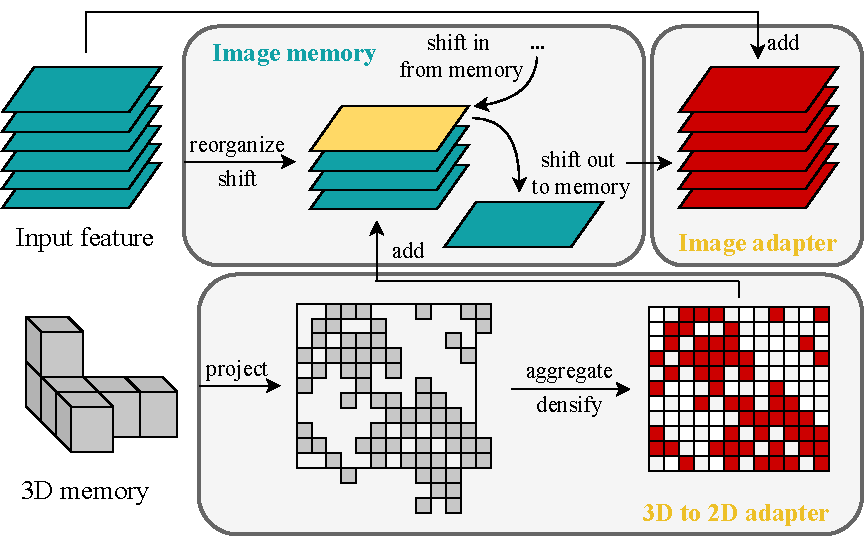
\includegraphics[width=1.0\linewidth]{figures/img-module-single.pdf}
    \caption{The architecture of the memory-based adapter for image features. We reorganize the input features and shift out a proportion of channels into the memory, while shifting in previous memory and aggregating temporal information by 2D convolution. We also resort to the 3D memory for more global context.}
    \label{img-module}
\end{figure}

\textbf{Memory construction:}
Different from 3D data where point clouds from different timestamps can be stored in a shared 3D space, for 2D data the image features are stacked into a streaming video.
A common practice to process this kind of data~\cite{kondratyuk2021movinets} is to maintain a queue and perform causal convolution (unidirectional along temporal dimension) to aggregate the information from previous frames to current image features. However, video analysis methods focus on extracting the global information of the streaming video up to now, while in our case we only need to enhance the current image features $\mathcal{M}_{I}(I_t)$. So causal convolution on previous frames will bring a large amount of redundant computation. 
Moreover, in online 3D scene perception, the most important information for image features is the observation of objects from multiple perspectives. Since an object is usually observed in a few adjacent frames, maintaining a short queue is enough in most cases.
To this end, we make an extreme simplification: we only store one frame of previous image and exploit temporal relations between frames at time $t-1$ and $t$.
In order to efficiently aggregate the adjacent frames, we adopt channel shift to cache the temporal information. Formally, given $\mathcal{M}_{I}(I_t)\in \mathbb{R}^{H\times W\times C}$, we learn a linear transformation $R_1\in \mathbb{R}^{C\times C'}$ to map the image features into another embedding space, where the first $\frac{1}{\tau}$ channels contain rich temporal information relevant to the next frame. Therefore the memory can be simply constructed by shifting out this part of channels:
\begin{gather}
    m^I_t=(\mathcal{M}_{I}(I_t)\cdot R_1)_{[:,:,:\frac{C'}{\tau}]}
\end{gather}
Note that this operation is repeated frame-by-frame, thus $m^I_{t-1}$ contains the temporal information relevant with current features $\mathcal{M}_{I}(I_t)$.

\textbf{Memory-based adapter:}
At time $t$, after shifting out a proportion of channels to memory, we can pad the empty channels with previous memory $m^I_{t-1}$. In this way, the temporal information of the adjacent two frames are merged into a single frame, for which we can directly adopt 2D convolution to aggregate the features:
\begin{gather}
    F_t={\rm 2D\text{-}Conv}(m^I_{t-1}\oplus(\mathcal{M}_{I}(I_t)\cdot R_1)_{[:,:,\frac{C'}{\tau}:]})\cdot R_2
\end{gather}
where $R_2\in \mathbb{R}^{C'\times C}$ is a learnable inverse transformation to map image features back to the original embedding space.
Finally we update $\mathcal{M}_{I}(I_t)$ by adding $F_t$ with a residual connection. We also zero-initialize $R_1$, $R_2$ and ${\rm 2D\text{-}Conv}$ for smooth finetuning.


\subsection{Inter-modal Temporal Modeling}
% 2d context-->inefficient
% 3d context-->in a shared 3D space, efficient, more context
% make use of 3d memory to enhance 2d feature
Although maintaining a short queue and adopting channel shift are able to effectively aggregate temporal information for image features, the global context is limited. This will lead to a performance drop when an object is very large or the RGB-D camera stops moving.
However, as analyzed before, extracting rich global context from a streaming video is really memory and computation consuming.
To solve this problem, we resort to the point cloud memory for global context extraction, because the point cloud features are efficiently cached in a shared 3D space and thus the length of queue can be long. We devise a 3D-to-2D adapter to refine current image features with the global 3D features.
Here we first project $m^P_{t-1}$ to the discrete image coordinate system with the inverse function of $\mathcal{S}$, which are then converted to sparse tensor. 
In this way, we keep the sparsity of point cloud memory and make the 2D features geometry-aware.
2D sparse convolution is then applied on the sparse tensor to aggregate the context information, followed by a densify operation to keep features inside image and pad other pixels with zero. 
Finally we add the densified 2D features to enhance $\mathcal{M}_{I}(I_t)\cdot R_1$ with richer global context. We zero-initialize the 2D sparse convolution for smooth training.

To acquire the final online perception results, a prediction fusion strategy is needed. As the focus of our work is the temporal learning modules for image and point cloud backbones, we only adopt a simple post-processing strategy to fuse the predictions of each frame in a whole, which we detail in Section \ref{impd}.

% \subsection{Prediction Fusion}
% The focus of our work is the temporal learning modules for image and point cloud backbones. Therefore we only adopt a simple post-processing strategy to fuse the predictions of each frame in a whole.

% \textbf{Semantic segmentation:} The predictions for each frame are concatenated, which has the same point number with $S_t$. We use 2$cm$ voxelization to unify the predictions for points inside the same voxel grid by channel-wise maxpooling.

% \textbf{Object detection:} The predicted bounding boxes for each frame are merged by 3D NMS. When two boxes of different time are colliding during NMS, we add $\delta$ to the classification scores of box in the newer frame. This is because our method ensures the backbone extracts more complete geometric features for the newer frame.

% \textbf{Instance segmentation:} Instance segmentation can be divided into transformer-based~\cite{schult2022mask3d}, grouping-based~\cite{jiang2020pointgroup,vu2022softgroup} and detection-based~\cite{hou20193d,yi2019gspn,kolodiazhnyi2023top}. As the first two kinds require a specially designed mask fusion strategy~\cite{liu2022ins} for online perception, we opt for the detection-based manner, where we can first conduct online 3D object detection and then utilize the boxes to crop and segment the point cloud features stored in the memory.

% More details can be found in supplementary material.